\section{ サヨナラは今もこの胸に居ます}

\parpic[r]{
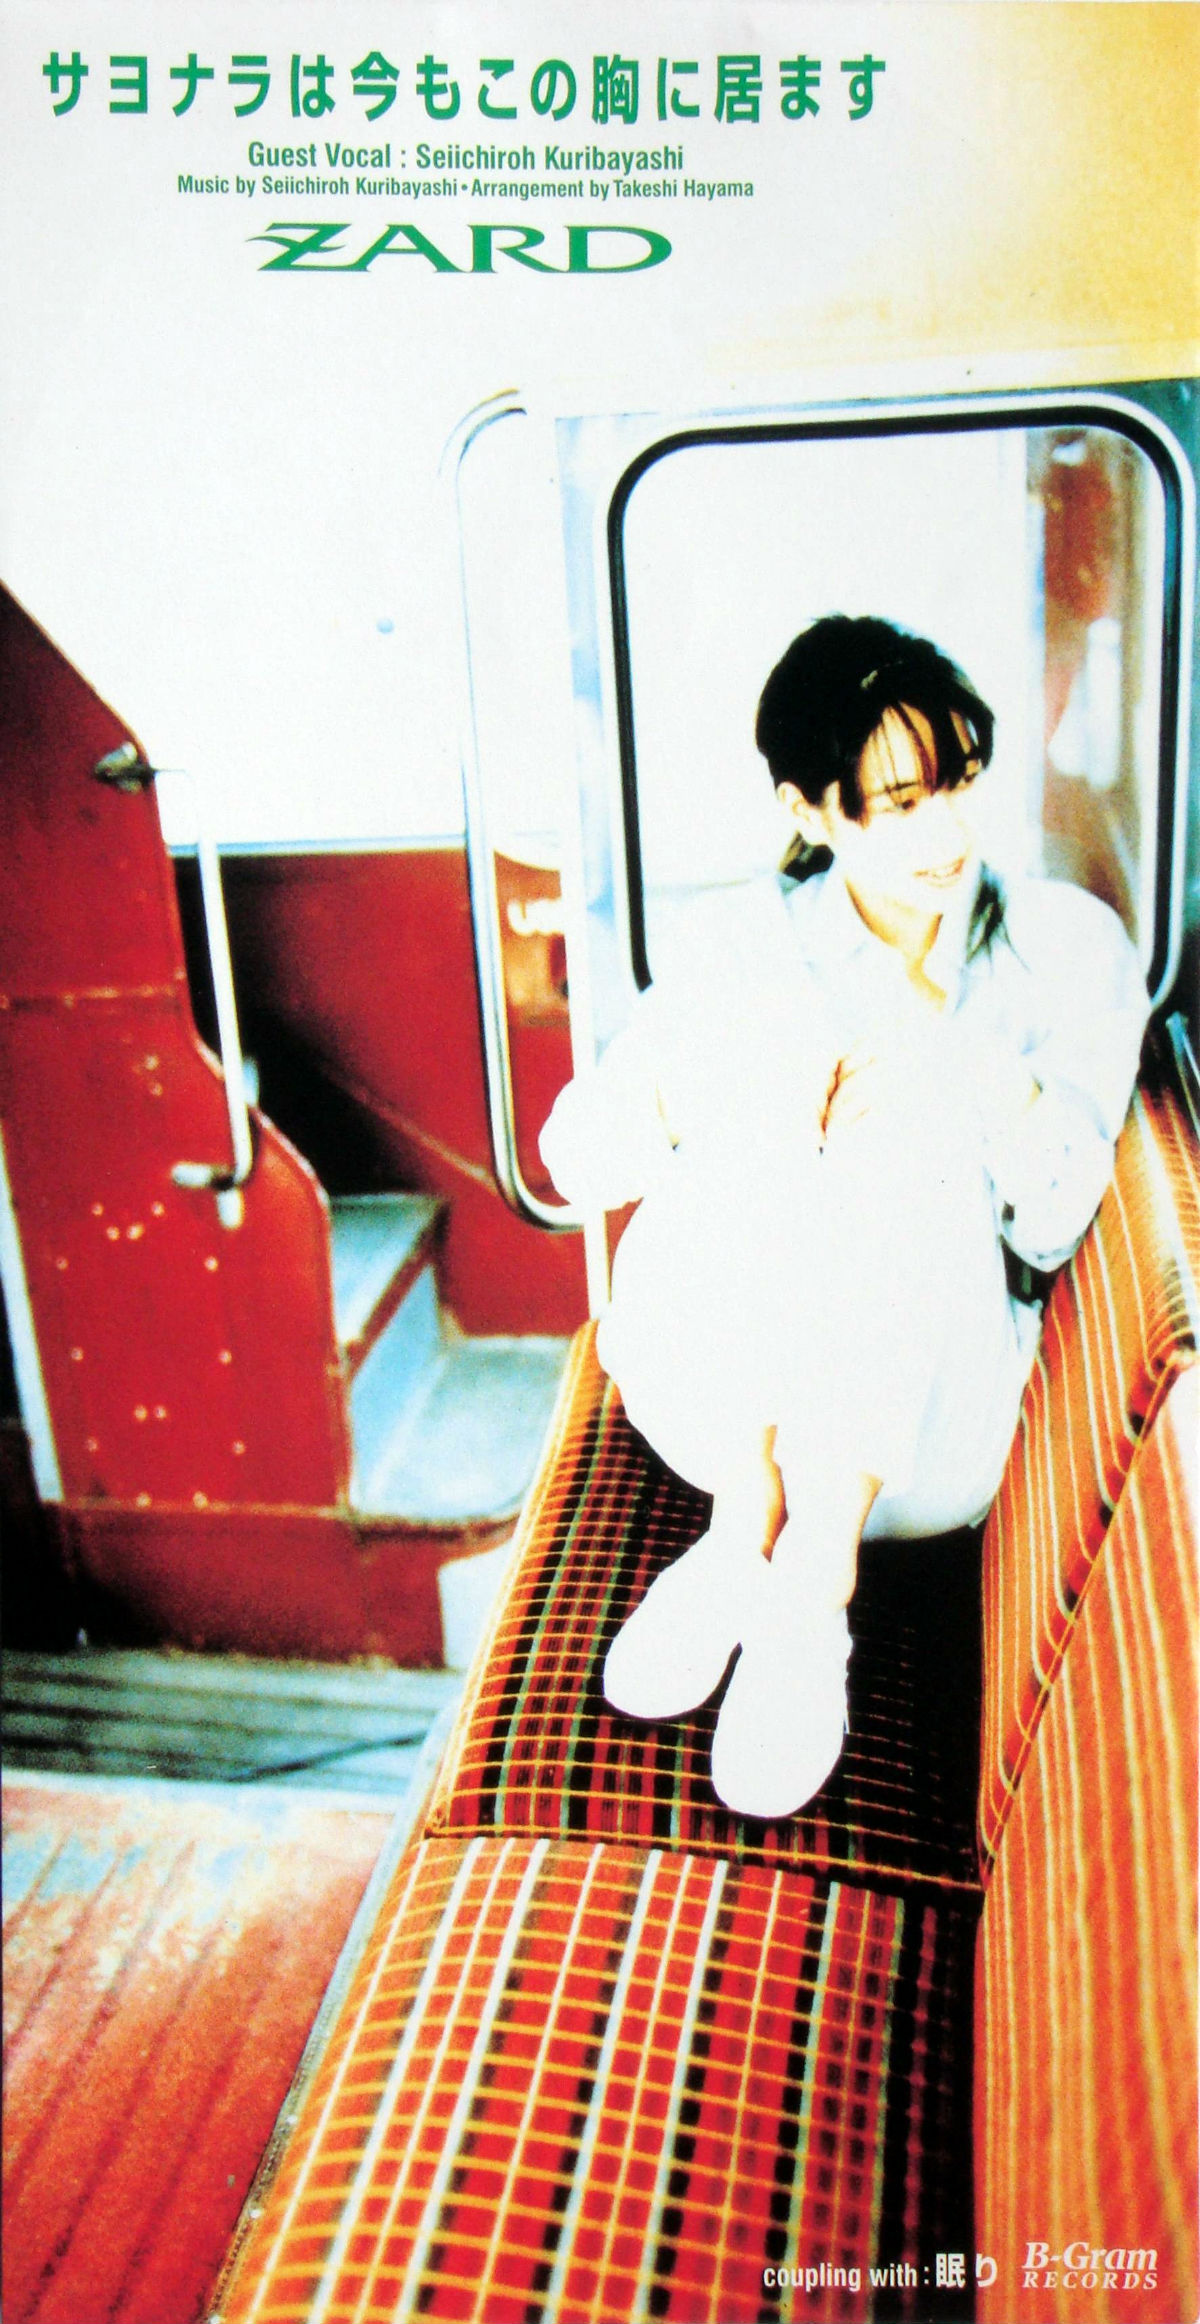
\includegraphics[width=0.3\textwidth]{S16.jpg}}

\large{

\ruby{地下鉄}{ちかてつ}の\ruby{駅}{えき}ひとつ\ruby{乗}{の}りすごし

\ruby{見慣}{みな}れた\ruby{街}{まち}を\ruby{横切}{よこぎ}ったら

\ruby{星空}{ほしぞら}を\ruby{数}{かぞ}える\ruby{頃}{ころ}あなたの\ruby{部屋}{へや}に\ruby{明}{あ}かりが…

もし あなたがいつか\ruby{独}{ひと}りになって

\ruby{私}{わたし}の\ruby{事}{こと}を\ruby{思}{おも}い\ruby{出}{だ}したら すぐに\ruby{連絡}{れんらく}してね

\ruby{好}{す}きだから\ruby{追}{お}わないと\ruby{心}{こころ}に\ruby{決}{き}めたの
\\

サヨナラは\ruby{今}{いま}もこの\ruby{胸}{むね}に\ruby{居}{い}ます

\ruby{出逢}{であ}った\ruby{頃}{ころ}の\ruby{私}{わたし}でいたい

あなたと\ruby{歩}{ある}いた\ruby{思}{おも}い\ruby{出}{で}の\ruby{中}{なか}を

\ruby{今}{いま}はひとり あの\ruby{道}{みち}をたどっています
\\

\ruby{久}{ひさ}しぶりにこんなに\ruby{笑}{わら}った

\ruby{笑}{わら}うことさえ\ruby{忘}{わす}れていた

\ruby{誰}{だれ}かに\ruby{必要}{ひつよう}とされたいから

\ruby{誰}{だれ}かの\ruby{為}{ため}に\ruby{ガンバ}{Gamba}ってる
\\

サヨナラは\ruby{今}{いま}もこの\ruby{胸}{むね}に\ruby{居}{い}ます

いつも\ruby{笑顔}{えがお}でかくしていたけど

\ruby{夏}{なつ}が\ruby{過}{す}ぎるたび この\ruby{胸}{むね}が\ruby{痛}{いた}い

\ruby{夜}{よる}はとても とても\ruby{長}{なが}く\ruby{感}{かん}じるのです
\\

サヨナラは\ruby{今}{いま}もこの\ruby{胸}{むね}に\ruby{居}{い}ます

\ruby{出逢}{であ}った\ruby{頃}{ころ}の\ruby{私}{わたし}でいたい

\ruby{楽}{たの}しかった\ruby{事}{こと} \ruby{苦}{くる}しかった\ruby{事}{こと}

そしていつの\ruby{日}{ひ}かあなたから\ruby{卒業}{そつぎょう}します

}